\chapter{Model}
\label{ch:model}

\begin{epigraph}
    \emph{For there is nothing lost, that may be found, if sought.} --- Edmund
    Spenser, \emph{Finding the Faerie Queene}, 1590.
\end{epigraph}



\reto{The model is one part of your contributions.
    Is it custom to have one contribution ready for your proposal?
    Shouldn't that go as 4.1 ?
}

\begin{quotation}
    \input{thesis.tex}
\end{quotation}

Testing this thesis requires an understanding of \emph{naming} and how I
envision pragmatics fitting as part of the larger naming model. As I have
pointed out when reviewing the background (\autoref{ch:background}) it is clear
that hierarchical models of naming were never intended to be the \emph{end} of
namespace development, though one could not tell that this is the case from
the storage systems that we use today.

The cracks have been showing for decades, the edifice of

\section{Naming}
\label{ch:model:sec:naming}

An essential part of my model is that it separates naming from storage: the
name does not need to incorporate the storage location.  This is not a new
observation, but it is one that is central to my thesis because addressing it is
an essential part of constructing the rich naming networks, which are central to
my thesis.

Thus, it is important to understand the fundamental purpose behind naming.
Salter'z work, which I describe in both \autoref{ch:introduction} and
\autoref{ch:background:sec:storage} captured the state of naming in 1978.  In
general, naming in 2021 is mostly the same as what Saltzer describes.

This paradigm is breaking down, however.  Recent popular press has discussed
that university instructors are now finding that students no longer understand
the folder/file
metaphor~\footnote{https://www.theverge.com/22684730/students-file-folder-directory-structure-education-gen-z}.
Instead, they have the \emph{laundry basket} metaphor, where all their content
goes into a small number of large collections.

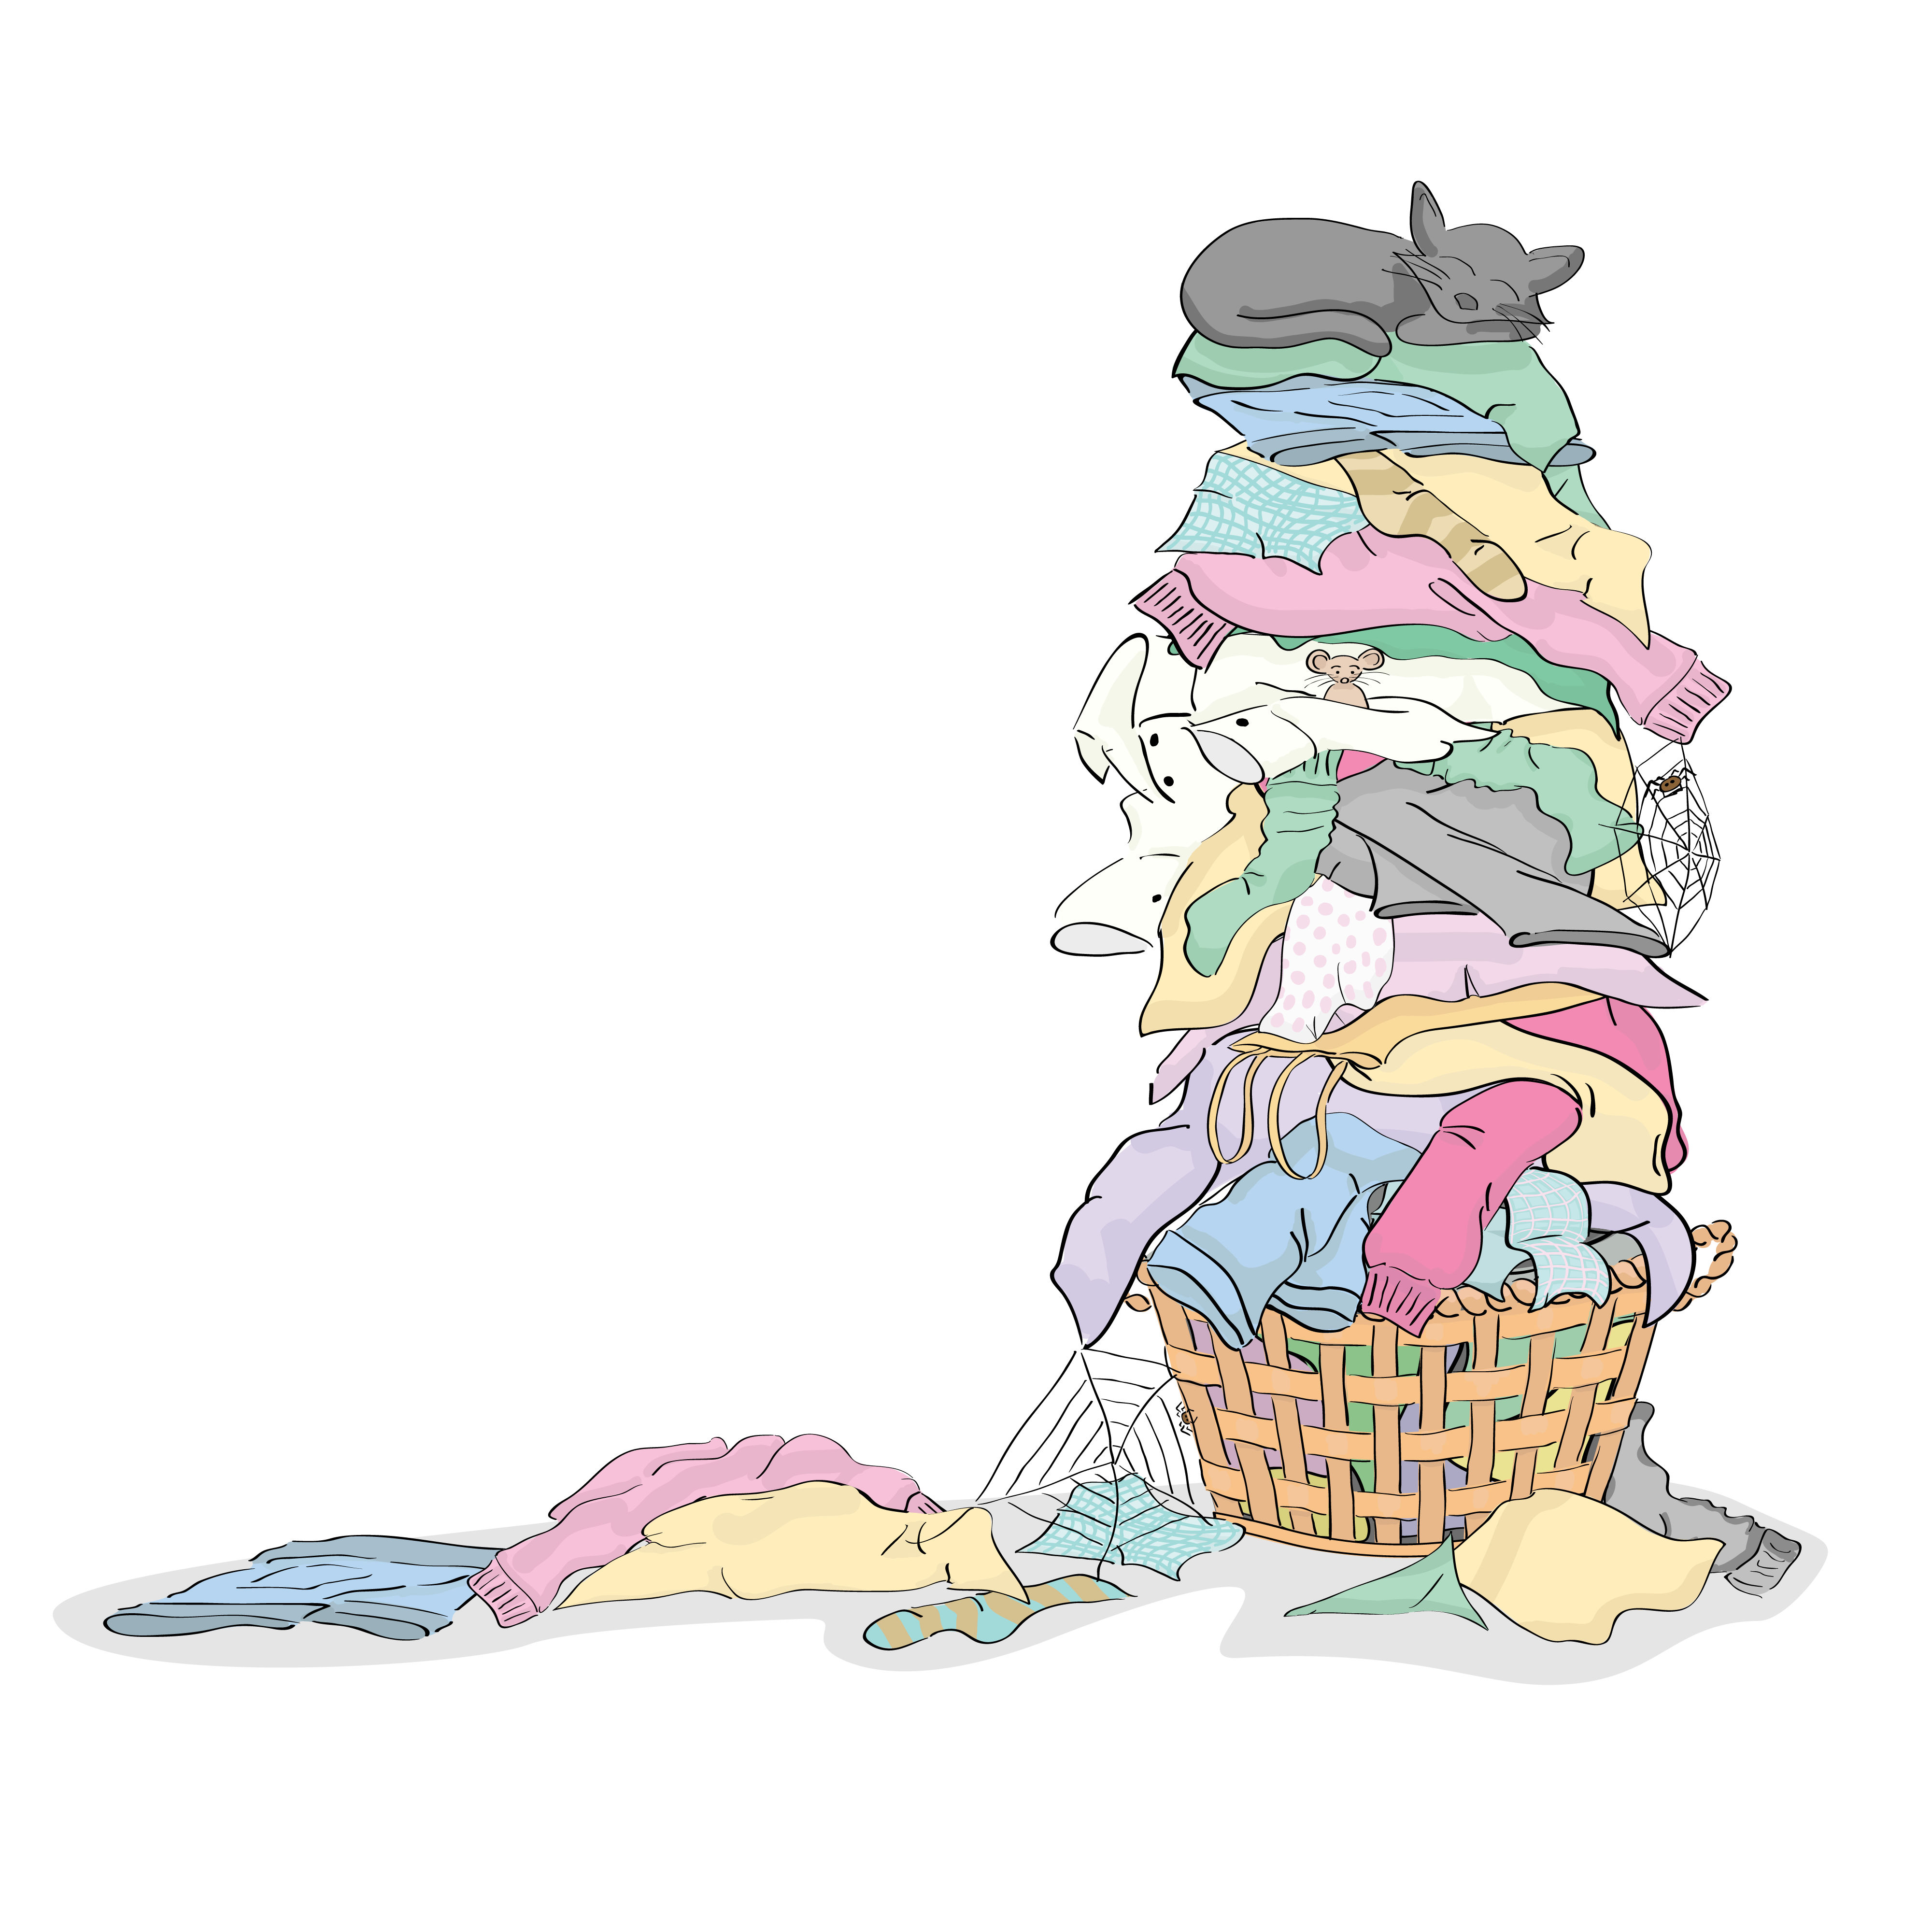
\includegraphics[width=0.95\textwidth]{figures/laundry-basket-with-cat-on-top.png}

Given the prior work, the fact the exiting folder/file paradigm has finally
broken down --- at least for the younger generation.  It \emph{also} suggests an
important way to consider my own thesis, namely can the introduction of
pragmatic naming prove useful to both those using the old paradigm of folder and
file, or the new paradigm of a laundry basket?

\begin{comment}
One challenge in developing this work is the resistance of the computer systems
community to considering \emph{naming} as a systems problem.  One common
response is to posit that this is an \ac{HCI} problem.  While there are
certainly aspects of data visualization that \emph{are} \ac{HCI} problems, a
review of the current state of affairs suggests this is clearly untrue.

\begin{itemize}
    \item The computer systems community has \emph{already} taken over at least
          some aspect of naming; it is dereliction of responsibility to now insist the
          current state of affairs is not tightly tied to earlier choices by the
          computer systems community.

    \item The \ac{HCI} community has been evaluating, reviewing, and proposing
          potential alternatives to the current computer storage naming paradigm
          for \emph{decades} but these solutions fall short of being viable because it
          is not sufficient to change a single application --- even something as core
          to the problem as the file browser --- to resolve this problem.

    \item The computer storage community does admit to the challenges here and
          have implemented system-specific solutions to improving naming, but human
          users do not live in a reality in which such narrow solutions resolve the
          naming challenges of the larger system --- it is not sufficient to argue
          that any storage system has solved this problem when users are called upon
          to use multiple storage systems on a daily basis.
\end{itemize}
\end{comment}

My survey of the background work (\autoref{ch:background}) makes it clear that
the hierarchical directory structure was not considered to be the best possible
naming system, but it was considered to be a reasonable first step.  Similarly,
we know from that prior work the embedding of location data within the human
naming scheme was not productive.

The problem has become untenable at point: it is now as easy to just hunt
through a large collection of files without hierarchical structure as it is to
try and organize them.  Search may be the correct answer, though Whittaker
certainly argues that it is not --- that humans prefer to \emph{navigate} than
search~\cite{bergman2019search,bergman2019factors}.  Perhaps this work is now
dated that younger computer users have themselves become uninterested in
hierarchical organization structure at all.

One problem with search currently is that there is no universal search.
The \ac{HCI} community has also observed that cross-silo storage has become the
\emph{reality} of most computer users~\cite{Thereska2013}: ``Through user
studies and measurements, we find that users and application developers
increasingly have to deal with a \emph{de facto} distributed system of
specialized storage containers/file systems, each exposing complex data
structures, and each having different naming and metadata conventions, caching
and prefetching strategies and transactional properties. First, there is tension
between the traditional local file system and cloud storage containers.
Local file systems have high performance, but they lack
support for rich data structures, like graphs, that other
storage containers provide. Second, distinct cloud storage
containers provide different operational semantics
and data structures. Transferring data between these containers
is often lossy leading to added data management
complexity for users and developers.''

The idea of separating the namespace from storage has previously been
suggested~\cite{mogul1986representing,placeless-tois}.  The concept of using
semantic meaning as part of naming is also not new~\cite{gifford1991semantic}.
However, much of this is \emph{inward focused} on the file itself.  The
attributes of the file (sizes and timestamps) or characteristics of the contents
of the file (semantic meaning).  Prior work has only lightly included the concept of
\emph{context} of how the files have been used, such as Placeless document's use
of the ``process''~\cite{dourish1999getting}.

Instead, my proposed concept of context is much broader: what \emph{else} was
happening within the system that might have been related to particular files:
``Show me code that I wrote while listening to \emph{Lie to Me} by Depeche
Mode.'' We might want to do that because the human mind works by association.
This was Bush's \emph{point} in his 1945 article: humans use associative context
to locate things.  This can then be used to augment other data sources,
including file meta-data, semantic information, tags, extended attributes,
properties, and any other existing forms of information that are available.
This rich data can then in turn be used to create various types of namespaces
including the ``virtual directories'' proposed by
Gifford~\cite{gifford1991semantic} but also to allow exploration of other
potential interfaces including faceted search and graph browser interfaces.

\section{Research Questions}
\label{ch:model:sec:research-questions}

\tm{Here is where I should put the research questions that I seek to answer,
    since those will drive the choice of models.
}

I consider the following research questions as part of evaluating my
thesis:

\begin{enumerate}

    \item \label{rq:pragmatics} Does adding \emph{activity context} improve
          associative access to files beyond the benefits of \emph{semantic
              context}~\cite{gifford1991semantic}.

    \item \label{rq:no-hierarchy} Given a cross-silo storage architecture, how
          do we allow existing applications built to rely upon an hierarchical name
          space to work properly? \tm{Maybe the right answer here are the virtual
              directories of Gifford, but I'm not sure that it is the right answer,
              either.  This question is likely too broad.}


    \item \label{rq:events} What system events are useful in establishing
          relationships between objects?

    \item \label{rq:hci} How can we provide the \ac{HCI} community with the
          additional contextual information they require to build better tools?

    \item \label{req:privacy} How can we provide distributed meta-data services
          while preserving privacy?

    \item \label{req:security} How do we allow securely sharing meta-data?

\end{enumerate}

\tm{Note that a dynamic list of the research questions is maintained at
    \url{https://wamason-my.sharepoint.com/:x:/p/tony/EYVA1mlCLd5HkftoizGx-ksBr6KodPWcg3bYq3e5mhwf4w?e=icUFtU}.
}


\section{\system Architecture}
\label{ch:model:sec:architecture}

\tm{This is where the model emerges.  I'll start with the Kwishut model and then
    work through it to ensure that it provides what I need to answer those research
    questions.
}

\subsection{Services}
\label{ch:model:sec:architecture:subsec:services}

\tm{TBD}

\endinput

\subsection{Computer Storage Naming}

\MIS{What is this? What am I getting and putting? It seems to me that there is a
    high level narrative missing: Different silos us different kinds of names: HNS,
    key-based put/get, keyword-based search (e.g., the web), I don't even know
    exactly what I would call github, hierarchical?  So the work here is figuring
    out what the categories of namespaces are, how they are similar, how they are
    different and why having many is a problem (e.g., if everything were simply
    explosed as mount points, multi-silos might not be a problem; we'd still have
    problems finding things, but not due to how names are constructed).
}

\tm{This is a placeholder for this information.  I need to figure out where the
    right place to put this is.
}

In addition, network namespaces have proliferated, often distinct, sometimes
providing an hierarchical interface (e.g., the \ac{FTP}) and sometimes providing
a key-value interface (e.g., the HTTP GET/PUT operations).  The proliferation of
disjoint naming silos makes it more challenging to find related information
across silos.  Even with an hierarchical name space there is no simple mechanism
for finding related information that is physically part of distinct silos
because the relevant portion of the namespace is tied to the corresponding
portion of the namespace.

Thus, the underlying location of a given data object is defined by its storage
silo. The hierarchical name space obscures this somewhat but the underlying
system is still a composite of the namespaces on existing storage.

Some of this is historical: the only reliable place where applications can store
context is within the fully qualified path name to a file.  While \emph{some} file systems
support extended attributes, while others do not.  Even file systems that do
support extended attributes have subtle challenges associated with them,
such as differing limitations on them across file systems, the fact they are
lost when moved between file systems that support extended attributes and file
systems that do not, and how, unlike other file system operations, there is not
even a somewhat uniform API for managing extended attributed.  UNIX-like systems
have the various ``xattr'' operations but Win32 applications on Windows have
only an indirect mechanism for managing them (via backup APIs) though Windows
has its own very different set of native system calls for reading, writing, and
enumerating extended attributes on file systems that do support them.

Thus, the most common solution is to use the file name to embed context
(``meta-data''). \tm{I thought this was one of the insight }


Using file names to
embed context (``meta-data'') is well-understood~\cite{guo2012burrito}.  Yet,
embedding context in file names does not solve the problem of storing dissimilar
types of data in the same location, which defeats the purpose of having
specialized storage.  Similarly, it does not solve the problem of placing data
objects in their optimal storage location while preserving their relationship.

\tm{I'm not sure I like this example, but I'll leave it here for the time being.}
The need for this is increasingly clear.  For example, Qumulo has created a
distributed file system by constructing a cross-silo hierarchical namespace
separated from actual storage location with predictive data migration to drive
better support for huge data collections. Qumulo's approach attempts to address
the cross-silo approach but continues to rely upon the hierarchical name space
to do so.

\begin{figure}[!tbh]
    \centering
    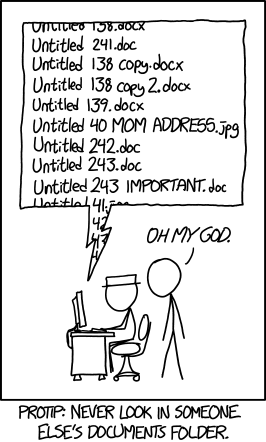
\includegraphics[height=5cm]{chapters/figures/xkcd1459.png}
    \caption{XKCD: Never Look in Someone Else's Documents Folder}
    \label{fig:xkcd:1459}
\end{figure}

Common types of file systems include:

\begin{description}
    \item[Media] --- such file systems manage persistent storage, such as solid
        state disk (``ssd''), rotating magnetic media (``hard disk''), magnetic
        tape, and rotating optical storage (such as a CD-ROM). Media file systems
        manage the data storage provided by the media device.  A media device can be
        constructed by combining portions of multiple media devices, such as is done
        with \ac{RAID} storage.  Media file systems also manage the correspondence
        between the file system's logical storage elements, which are typically files and
        directories, and

    \item[Network] --- such file systems utilize a network protocol for
        transferring data from one or more computers accessed across a network so
        that it can be consumed by local applications.  Examples of network file
        systems include \ac{NFS}, \ac{AFS}, and \ac{CIFS}. Network file systems
        manage moving data between computer systems over the network, presenting a
        compatible name space, and manage data caches and coherence between local
        caches and remote storage.  Sometimes these are also referred to as
        \emph{distributed} file systems.

    \item[Pseudo] --- such file systems provide structured information extracted
        from non-storage locations and present it via an hierarchical name
        space.  For example, the \emph{proc} file system (\tm{From Plan 9?})
        presents information about the running operating system.  A pseudo file
        system manages its namespace as well as retrieving or storing data that
        relates to the corresponding system state.

\end{description}


\tm{Note that this is the point at which I have stopped during the re-write of
    this section.  Content beyond this point is being reworked.
}




In \autoref{ch:background:sec:challenges} I attempted to capture key aspects
of how naming is used by human users and from that proposed a basic list of key
elements to consider in a comprehensive naming model: identity, location,
relationship, characteristic, and context.  While this is a good place to begin
my analysis, more is needed to construct a robust model.  For example, one of the
challenges of naming is that it is \emph{dynamic}: the storage
location of a given data object might change.  This often means that the
\emph{name} also changes, because the name encodes location.  This is no more
intuitive to a human than it would be to insist someone change their name each
time they moved to a new home.

In other words, the \emph{object} is not different even though its storage
location changes.  Neither users nor applications care about this
specific detail until they go to actually retrieve it.  In the current model,
rather than bein forwarded to the correct object an error is returned indicating
that the object is no longer accessible.

To facilitate developing my naming model, I rely upon several use-cases that
have arisen during the course of my research around this topic, both working
with collaborators as well as discussions for ordinary users that are unfamiliar
with my research area. \tm{Margo suggested that I be specific here by pointing
    to particular people in footnotes for the time being.  I defer that for the
    moment but it is a good thing to add as I continue editing.}

\section{Use Cases}
\label{ch:model:sec:use-cases}

%%%%%%%%%%%%%%%%%%%%%%%%%%%%%%%%%%%%%%%%%%%%%%%%%%%%%%%%%%%%%%%%%%%%%%%%%%%%%%%%%%%%%%%%%%%%%%%%%%%%%%%%%
\begin{table*}[!tbh]
    {\renewcommand{\arraystretch}{1.3} %<- modify value to suit your needs
        \begin{tabular}{p{0.2\textwidth}p{0.4\textwidth}p{0.4\textwidth}}
            \hline
            \textbf{Feature}                                                                                                                                        & \textbf{Existing Technologies} & \textbf{No Solution} \\
            \hline
            \usecaseactivitycontext                                                                                                                                 &
            timestamps and geo-location, image recognition, browsing history, ticketing systems, application-specific solutions like Burrito~\cite{guo2012burrito}. &
            Link related activity across apps, record  browsing history and chat conversations relevant to the creation of the data object, storing it in ways that are secure and compact.
            \\
            %
            \usecasecrosssilosearch                                                                                                                                 &
            Search by name, creator, content across silos,
            app-specific searches (e.g., Spotlight)                                                                                                                 &
            Unified search across all kinds of storage, including file systems, object stores, apps and devices
            \\
            %
            \usecasedatarelationship                                                                                                                                &
            De-duplication of documents, versioning of specific files, git ancestor relation                                                                        &
            Explicit notion of data identity, tracking different versions across different silos as data is transformed
            \\
            %
            \usecasenotifications                                                                                                                                   &
            File watchers (INotify), synchronization status, manually inspecting modified time                                                                      &
            Ability to subscribe to specific changes on attributes
            \\
            %
            \usecasepersnamespace                                                                                                                                   &
            Hierarchy plus hard/soft links. Use of tags.                                                                                                            &
            Creating personalized namespaces with with flexible data organization and views
            \\
            \hline
        \end{tabular}
    }
    \caption{Use-case driven functional requirements.}
    \label{tab:usecases}
\end{table*}
%%%%%%%%%%%%%%%%%%%%%%%%%%%%%%%%%%%%%%%%%%%%%%%%%%%%%%%%%%%%%%%%%%%%%%%%%%%%%%%%%%%%%%%%%%%%%%%%%%%%%%%%%

To motivate the model I propose for \system, I first start with a series of
potential use cases. \tm{Note that I've started with the two from the original
    \system paper, but I think it might be worthwhile to add one or two more to
    provide a more well-rounded model.}

\begin{description}
    \item[Data Processing]
    \item[Compliance]
    \item[Memex]
    \item[Asset Management]
\end{description}

Using these uses cases as motivation, I propose that \system support the
features as shown in \autoref{tab:usecases} in greater detail in \autoref{ch:model:sec:features}.

\subsection{Data Processing}
\label{ch:model:sec:use-cases:subsec:data-processing}

\tm{This is from the HotStorage paper submission}

\persa and \persc are preparing a report summarizing their work on a data analysis project for a customer.
\persc sends an email to \persa containing a CSV file with original data.
\persa opens this document in Excel, formats and filters it, adds additional data from a corporate storage silo,
and then returns the Excel document to \persc on Slack.
\persc is away from their desk when it arrives, so they open it on their phone, uploading it to a cloud drive.
\persc then sends the link to \persa for editing with update notifications.
Finally, \persc sends a PDF of the report to the compliance officer who promptly asks, ``Where did this data come from?''

\subsection{Compliance}
\label{ch:model:sec:use-cases:subsec:compliance}

\noindent\textbf{Delete Request:~}
Some time later, the compliance officer requests that all documents containing a customer's data must be deleted.
To help with finding all relevant customer data, \persb joins the project and examines the report and requests the original data from which it was produced.
\persa remembers that they gave the original data to \persc shortly after
collecting it, but does not remember the name, location, or even how the
relevant files were transmitted. Thus, \persa has to manually search possible
locations and applications, sensing references to documents to \persb, who then
starts organizing these files to methodically identify the ones that might
contain the customer's data. In the process, many of the other team members'
references to the documents stop working.

\tm{
    Discussion with Ada: how do people do this \textit{already}?  Why are those
    solutions insufficient?  Some sites are accessible and others are not.  How
    do they \textit{prove} they are GDPR compliant?  What about when people move
    from dynamic to static memory?  Could I use storing the hash value as a
    mechanism for motivating this because it facilitates finding things.  Much
    like the Apple content hash for child p0rn.  How about extracting text from
    pictures to avoid censorship?
}

\MIS{
I think the current answer is 'not very well' -- it's an area of current
research and right now, I'm 95\% certain that aggregated data that was
influenced by individual data gets ignored. [Michael is just now submitting
a paper with MSR and Mickens on how to do better, but it's not like there
are solutions; instead people use a very narrow definition of what a user's
data really is.
}

\subsection{Memex}
\label{ch:model:sec:use-cases:subsec:memex}

The ``memex'' is a device posited by Vannevar Bush in 1945~\cite{bush1945we}:

\begin{quotation}
    \emph{``Consider a future device for individual use, which is a sort of mechanized
        private file and library. It needs a name, and, to coin one at random,
        "memex" will do. A memex is a device in which an individual stores all his
        books, records, and communications, and which is mechanized so that it may
        be consulted with exceeding speed and flexibility. It is an enlarged
        intimate supplement to his memory.''}
\end{quotation}

While the world wide web is certainly one interpretation of his forward thinking
article, the system he describes is also highly personal and appears to focus
not only on finding things but also capturing the context in which they are
found.

\tm{Seems like the key here is to extract the salient factors that would impact
    this model.  Note that \emph{context} is a remarkably critical element of
    understanding language in general, and naming particularly.  In Linguistics,
    they study \emph{pragmatics}, which are distinct from \emph{semantics}, and
    an important aspect of this is the context in which something --- including
    a name --- is used.  I need to explore this aspect of linguistics further
    because I have this sense that understanding the gap between the two naming
    systems is helpful in understanding why computer storage falls short.
}

Thus, when considering my naming model, I can draw upon the needs of Memex to
assist in ensuring the model is sufficient to meet the issues raised by
Bush~\cite{bush1945we}:

\begin{description}
    \item[Selection] --- ``The prime action of use is selection, and here we are
        halting indeed.'' The key here is being able to \emph{filter} items of
        interest at a given time. This becomes important as the number of objects
        being considered grows.  While computers are somewhat faster than they were
        in 1945, he points out the general problem of scaling and the need to be
        able to limit the actual size of the search space.  This is a very real
        consideration for our naming system: scalability.  Brute force search is not
        sufficient, as that is what we have \emph{now} and even as fast as storage
        systems are today this is not tenable.

    \item[Association] --- ``Our ineptitude in getting at the record is largely
        caused by the artificiality of systems of indexing. When data of any
        sort are placed in storage, they are filed alphabetically or numerically, and
        information is found (when it is) by tracing it down from subclass to
        subclass. It can be in only one place, unless duplicates are used; one
        has to have rules as to which path will locate it, and the rules are
        cumbersome. Having found one item, moreover, one has to emerge from the
        system and re-enter on a new path.

        ``The human mind does not work that way. It operates by association. With one
        item in its grasp, it snaps instantly to the next that is suggested by the
        association of thoughts, in accordance with some intricate web of trails
        carried by the cells of the brain. It has other characteristics, of course;
        trails that are not frequently followed are prone to fade, items are not
        fully permanent, memory is transitory. Yet the speed of action, the
        intricacy of trails, the detail of mental pictures, is awe-inspiring beyond
        all else in nature.''

        Thus, the key take-away here is to find associations.  This is part of
        the motivation for \emph{activity context}.

    \item[Trails] --- ``And his trails do not fade. Several years later, his
        talk with a friend turns to the queer ways in which a people resist
        innovations, even of vital interest. He has an example, in the fact that the
        outraged Europeans still failed to adopt the Turkish bow. In fact he has a
        trail on it. A touch brings up the code book. Tapping a few keys projects
        the head of the trail.''

        Thus, the key take-away here is to be able to show at least one kind of
        relationship: a ``trail,'' which seems to be similar to provenance.

\end{description}



\subsection{Asset Management}
\label{ch:model:sec:use-cases:subsec:asset-management}

One recurring theme in my conversations with the visual arts community, has revolved
around the management of \emph{assets}. This term is broadly used: web pages are
constructed of assets such as text, graphics, style sheets, and XML schema, all
of which are combined together to form a unique view of the given web page that
is relevant in the specific context of the viewer who may be using a graphical
computer, smartphone, tablet, or text-based web browser.

Similarly, computer games combine their own version of assets. Unity is a highly
popular framework for constructing interactive computer games and their website
defines an asset: ``Shorthand for anything that goes into a video game ---
characters, objects, sound effects, maps, environments,
etc.''~\footnote{https://unity.com/how-to/beginner/game-development-terms}

There is no single hierarchical organizational structure for assets that
satisfies the needs of this type of creative endeavor: a single game asset could
be classified by a myriad of characteristics.  When a game developer is looking
for a particular asset, they are often focused on those characteristics.  When
an audio engineer is attempting to construct specific sound effects they could
be looking for: the duration, number of channels, channel mapping, sampling
frequency, bit depth, instrument, or dynamic range for example.  It is clear
that what doesn't work in such a situation is a single directory filled with all
of the assets: that isn't useful.

Indeed, this use case seems to focus on being able to identify and use the
\emph{properties} of a given data object.  Simpler examples of this might be how
one organizes documents for accounting purposes: bank statements could be sorted
by the bank from which they came or the month that they cover.  In my
experience, accounting users actually will store copies of such a file because
they need to be able to identify it in \emph{both} formats.  Another similar
example is ``how do you organize your music collection?''  A music collection
could be organized by artist, or album, or year of release, or publisher or
lyricist, or genre. When we have a physical copy of recorded music (e.g., an
eight-track tape~\footnote{Invented in 1964 and thus as old as Multics, which
    adopted the hierarchical file system structure.} we are limited to the ways in
which we can organize it.  Digital files have no such limitations; that
limitation is an artifact of the current naming system.

\tm{What requirements are imposed by this use case?  It's relatable, but does it
    really impact the design?
}

\section{Features}
\label{ch:model:sec:features}

\system must provide the following features to meet the needs of the use cases:

\begin{description}
    \item[Activity Context] --- this is a mechanism by which we capture
        information for understanding the context in which data is created,
        transformed, and accessed.  This is not application or storage silo specific
        information. Examples of this might include timestamps, application specific
        meta-data, history information, provenance information, etc.

    \item[Search] --- while search is not the only use we envision for \system,
        it is one of the mechanisms that we expect to enable and should support
        searching across storage silos and exploiting the richer meta-data
\end{description}

\section{Architecture}
\label{ch:model:sec:architecture}

\tm{I'm starting with the \emph{Kwishut} architecture from HotStorage 2021.}

\begin{figure}[!tb]
    \centering
    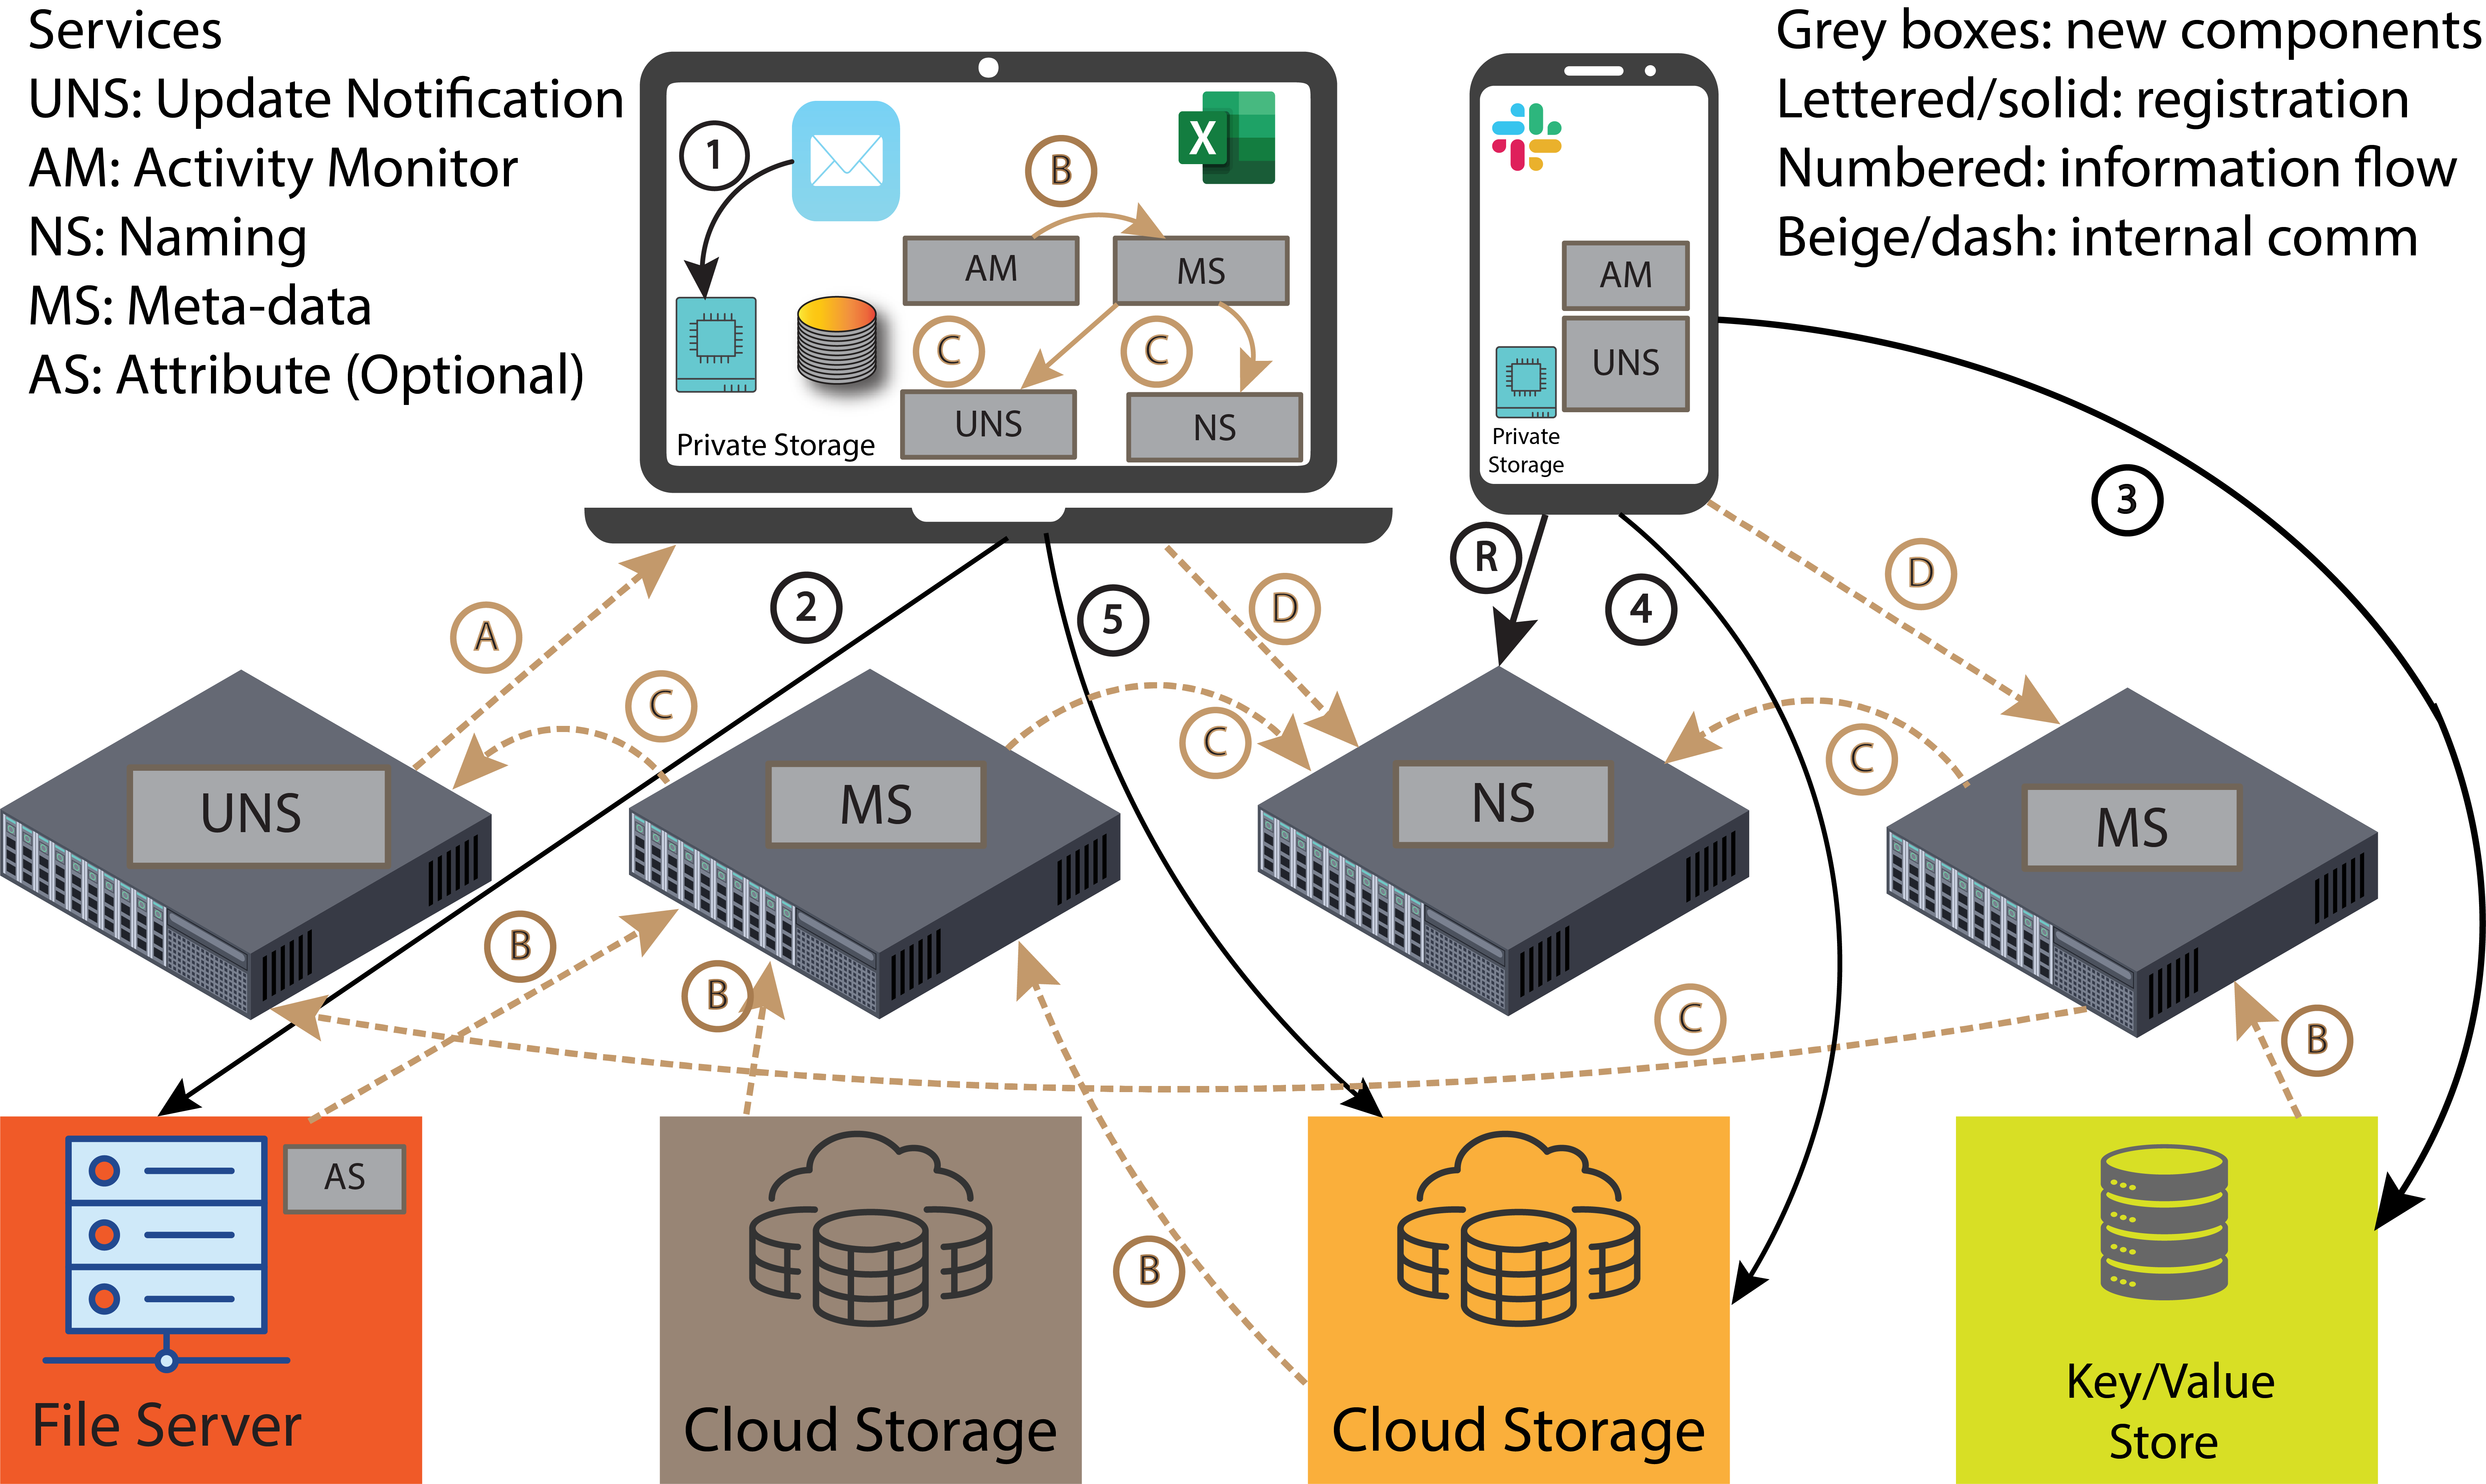
\includegraphics[width=0.45\textwidth]{reference/hotstorage21/figures/Naming5-legend.png}
    \caption{\emph{\system} Architecture (see \autoref{ch:model:sec:architecture:subsec:services}).\\%
        Grey boxes indicate new components. AM=``Activity Monitor'', MS=``Meta-data Server'', UNS=``Update Notification Server'', NS=``Namespace Server''.
    }
    \label{ch:model:fig:arch}
\end{figure}

%\reto{Using meta-data service that must inter-operate (federated meta data) and relationships are not first-class citizen, cannot glue the meta-data service together with naming services to enable the things we want to do. }
%\reto{the storage location is independent on the notion of related files: meta-data service treats relationships as first-class citizens. }
%\reto{get the attributes out of the silos --> currently: this is done manually}

\emph{\system} is a family of services that enable sophisticated search and naming capabilities.
The key features that differentiate \emph{\system} from prior work are:

\begin{enumerate}[1)]
    \item incorporating object relationships as first class meta-data because
          prior work has not done so which interfers with the ability to ensure
          meta-data and naming services work together; and
    \item federating meta-data services, which is necessary to ensure
          efficiency, scalability, and security; and
    \item recording activity context, which is necessary to provide insight into
          how the data is used dynamically (over its lifetime) rather than statically
          (at the point of creation or last update); and
    \item integrating storage from multiple silos, which is necessary to clearly
          distinguish the storage characteristics that are focused on storage service
          optimization from the usage characteristics that establish associative
          context; and
    \item enabling customizable naming services, which are needed because we
          need the flexibility to support a broad range of existing as well as
          innovative new storage services.
\end{enumerate}

Data continues to reside in existing and to-be-developed storage silos.
\emph{\system} interacts with these silos, collects and captures metadata, and
provides a federated network of metadata and naming services to
meet the needs of users with the use cases in \S \ref{tab:usecases}
being our initial evaluation of our architecture and design.

\subsection{\emph{\system} Services}
\label{ch:model:sec:architecture:subsec:services}

Figure \ref{ch:model:fig:arch} illustrates the \emph{\system} architecture. \emph{\system} allows for
different deployment scenarios. The services can be run independently, they
can be co-located and bundled together to run on a local device, integrated into
an OS, or available as network-based services.

In the discussion below, parenthesized numbers and letters refer to the arrows
in Figure \ref{ch:model:fig:arch}. There are five main components:

\begin{enumerate}[1)]

    \item \textbf{Metadata servers (MS)} are responsible for storing attributes
          and provide a superset of capabilities found in existing metadata
          services~\cite{federatedMetaData,smartstore}. Users can register an MS with
          activity monitors or attribute services, which allows the MS to receive
          updated attributes from storage objects and activities (B). Thus, there can
          be multiple sources of attributes including the user itself. Metadata
          servers may retain the full or partial history of attribute updates or
          maintain only the most recent value.

    \item \textbf{Namespace servers (NS)}
          connect to one or more MS and use the metadata to provide users with a
          personalized namespace that allows both manual organization (i.e., a
          hierarchical namespace) and rich search capabilities.
          Users can register with an NS (R) that uses one or more MS to obtain relevant
          attributes from them (C). Additionally, users can be part of a corporate NS that
          allows sharing of their select metadata with other users via standard enterprise
          public-key cryptography.

    \item \textbf{Activity monitors (AM)}
          run on the user's devices. Their main function is to observe temporal relations,
          activity context, and relationships between objects on a user's device and
          transmit them to an MS (D).


    \item \textbf{Attribute services (AS)}
          extract attributes from storage objects and transmit them to an MS (B). An AS
          might be invoked on updates, run once or periodically. For example, a file
          system AS would update the object's metadata with basic attributes such as size
          or modification time. There can be many AS that extract more ``interesting''
          attributes, e.g., image recognition, similarity, or other classifiers.

    \item \textbf{Update notification server (UNS)}
          provides notification mechanisms. Users can register interest in changes of
          attributes or underlying storage and will receive a message on change events (A)
          to which they have access.

\end{enumerate}

\subsection{\emph{\system} working example}


To make the \emph{\system} architecture concrete, we revisit our use-cases from
\S\ref{tab:usecases} and walk through parts of it to illustrate how \emph{\system}
supports the various actions and events.

\noindent\textbf{Storing the e-mail attachment.}
\persa's act of saving the CSV file that \persc sent in email corresponds to the
creation of a new object on the file server silo, i.e., the file system (4). The
file server is \emph{\system}-aware, so the AS co-located with it extracts
attributes from the document and forwards them to the MS (B).

The AM on \persa's laptop detects that the CSV file came via company email from
\persc. It then captures the activity context identifying the relationship
between the e-mail and the CSV file and transmits it as additional metadata
about the CSV file to the MS (that already contains metadata extracted by the
AS). Moreover, because there is a company-wide namespace service, \emph{\system}
establishes that the e-mail attachment, the CSV in the file server, and the one
on \persc's laptop (from which the file was sent) are exact copies of each
other.

Many applications already record some form of activity context, e.g., chat
history, browsing history. Such histories provide a rich source of additional
metadata. Other activity context, specifically the relationship between objects,
such as the fact that a particular file was saved to a local storage device from
an email message, requires more pervasive monitoring as found in, e.g., whole
provenance capture systems~\cite{camflow}. \emph{\system} is agnostic about the precise
data that comprises activity context, but allows for storing and accessing
activity context as metadata.

\noindent\textbf{Creating the Excel file.}
Next, \persa opens the CSV file using Excel and stores it as a spread sheet.
This creates a new object. The AM detects that the newly created spreadsheet is
a conversion from the CSV file, either via a notification from \emph{\system}-aware
Excel or by monitoring the system calls executed on the local system. \persa
proceeds to modify the data by filtering it in Excel and saving the changes. The
AM records this event and updates the meta-data of the spreadsheet to record the
derivation-relationship. Ideally a \emph{\system}-aware version of Excel specifies to
the AM the exact type of the relationship (in this case a derivation); otherwise
the AM informs the MS about an unspecified data relationship by observing the
opening of a CSV file and a subsequent creation of the Excel file.

% \persa proceeds to upload the new Excel file on Slack, which triggers the creation of a new storage object as Slack creates a local copy, the addition of new metadata to MS via AS, and the addition of a \emph{copy} data relationship between the original Excel file and the Slack’s copy. The AM notices (by monitoring Slack chat) that the file was shared with user \persc and promptly notifies the MS, which adds this detail to its metadata.
% Once \persa is done, its local MS has been updated with three new objects: the CSV file, the corresponding Excel file, and Slack’s copy of the Excel file. There is a data relationship linking all three, and the metadata informing us that the original CSV came from \persc and that the final Excel file was also shared with that same person. If \persa wanted to remember what happened to the the data from the original CSV from \persc, they could query their local personal NS, which would track down this history by querying the MS metadata.

\noindent\textbf{Sharing the spreadsheet.}
As \persc  receives the Excel file from \persa via Slack on their phone, a
sequence of metadata events similar to those described earlier takes place,
except the phone does not run a local NS or MS. \persc now uploads the file to
the company's cloud drive (4). The MS (by way of AS) reflects the creation of a
new object and records its remote location. The use of a company-wide namespace
and metadata service enables \emph{\system} to record that the file in the cloud drive
is, in fact, a copy of the one received via Slack.  Further, \persc informs
their personal NS that they wish to notify \persa about all updates to the file
on the cloud drive. Thus, whenever an AS sends updated attributes to the MS,
\persc receives a notification.

% The sharing relationship between the personal NS of \persa and \persc, and the exchange of the relevant cryptographic credentials, would have been set up earlier.

\noindent\textbf{Data origin and delete requests.}
When the compliance officer asks about the origin of the data, \persc can query
the corporate NS to obtain the complete history of the report. This includes the
spreadsheet from which the report was derived and the e-mail or Slack messages
that transmitted the files.
The corporate NS was configured to be aware of the locations of the
collaborating users' personal NS. Moreover, because of the activity contexts
captured by the AM, \emph{\system} is able to identify documents that were created
during any activity involving the customer whose data must be deleted. Starting
from these documents, and by using the relationship of documents, \persb was
able to find all relevant objects and delete them, including the e-mail and
Slack messages.


% \persa would have configured their personal NS to allow sharing of the metadata associated with \persc with their corporate NS, and \persc would configure their personal NS similarly. As a result, when \persc issues to the corporate NS a query asking to trace the origins of the data in the final report, the corporate NS is able to return all the history tracing back to the original CSV file.

Note that unlike existing systems, \emph{\system} is able to efficiently find related
objects across storage silos. Operating systems already provide users with
indexing services to accelerate search of local files. This search can be made
cross-silo by mounting and enabling indexing on network shares (e.g., Windows
Desktop Search), or by interfacing with specific applications such as e-mail
(e.g., MacOS Spotlight, or Android search). The problems with indexing on a
large network storage repository are resource limitations such as bandwidth and
local storage that may render the system unusable during indexing. In contrast,
\emph{\system} addresses these limitations by delegating indexing and storage to one or
more services.

NS are responsible for providing efficient search functionality. \emph{\system} uses AS
to keep attributes up to date with object modifications. Lastly, \emph{\system}
supports coordinated search among one or more local and remote NS, allowing, for
example, a user to search across both their local NS as well as their employer's
NS.

\tm{Would it be useful to resurrect some of the excluded text from this section?}
